\documentclass[11pt,a4paper]{article}
\usepackage[T1]{fontenc}
\usepackage[utf8]{inputenc}
\usepackage{lmodern,microtype,amsmath,amssymb,amsthm,booktabs,tabularx,tikz}
\usepackage[a4paper,margin=27mm]{geometry}
\usepackage[section]{placeins}
\usepackage[hidelinks,pdftitle={Conservación de la aleatoriedad de un PTG.2 mediante AES/SHA y CTR_DRBG}]{hyperref}
\usetikzlibrary{arrows.meta}
\renewcommand{\abstractname}{Resumen}
\renewcommand{\figurename}{Figura}
\renewcommand{\tablename}{Tabla}
\renewcommand{\refname}{Referencias}
\renewcommand{\proofname}{Demostración}
\newtheorem{proposicion}{Proposición}
\newcommand{\Enc}{\operatorname{AES}}
\newcommand{\HH}{\operatorname{SHA256}}
\newcommand{\bits}{\{0,1\}}
\newcommand{\cat}{\mathbin\Vert}
\newcommand{\upd}{\operatorname{Update}}
\newcommand{\leanlink}[2]{\href{https://github.com/jordiprga/technical-work/blob/8fec7ab9275547be9d74f394aa4fecbd86a13903/operation-token-burn-2026-11-14/00_coordination/ptg3-its/formal/Composition.lean\#L#1}{\texttt{#2}}}
\tikzset{op/.style={draw,inner sep=5pt,align=center,font=\small},arr/.style={-{Stealth[length=1.8mm]},thin}}
\raggedbottom
\title{Conservación de la aleatoriedad de un PTG.2\\ mediante AES/SHA y CTR\_DRBG}
\author{}
\date{27 de noviembre de 2026}
\begin{document}
\maketitle
\begin{abstract}
Se estudian dos procedimientos de posprocesamiento con estado para la salida de un generador físico PTG.2 con extracción Toeplitz. El primero emplea el DRNG AES/SHA de los §§996--998 de AIS 20/31 v3.0. El segundo emplea CTR\_DRBG AES-256 sin función de derivación, con una entrada adicional de 384 bits cuyos 128 bits inferiores contienen la palabra física. Para ambos se especifican la inicialización, la generación y la actualización del estado. Se demuestra que, fijado el estado inicial, cada procedimiento permuta las secuencias de bloques completos de 128 bits. Por ello se conservan la distancia a la distribución uniforme y la minentropía condicional frente a la misma información lateral. La demostración depende de la invertibilidad de AES y se distingue de los argumentos computacionales exigidos para DRG.3. Se identifican el precedente explícito de AIS para AES/SHA y las obligaciones pendientes del perfil CTR.
\end{abstract}

\section{Modelo y notación}
Un PTG.2 es un generador físico de números aleatorios de la clase definida en AIS 20/31 \cite{ais}. En la arquitectura estudiada, el PTG.2 entrega un flujo de bits después de la extracción Toeplitz. Se toma como premisa la garantía teórico-informacional (ITS, \emph{information-theoretic security}) de ese flujo. Para un horizonte especificado, la distribución conjunta de los bits extraídos está a distancia a lo sumo \(\varepsilon\) de una distribución uniforme independiente de la información lateral considerada. El análisis comienza en la salida del extractor. El objetivo es determinar qué garantía se mantiene al añadir un generador determinista con posprocesamiento criptográfico.

El \emph{material de siembra} es la cadena de bits que consume el procedimiento de inicialización. El \emph{estado inicial}, denotado por \(S_0\), es el conjunto de valores guardados por el generador al concluir ese procedimiento, antes de la primera salida. Un registro en hardware o un campo de una estructura en software puede conservar esos valores entre dos operaciones. En AES/SHA el estado es una clave de 256 bits. En CTR\_DRBG el estado de trabajo comprende una clave, un contador criptográfico y un contador administrativo. El procedimiento de inicialización determina la relación entre el material recibido y los valores que quedan en esos registros.

Una \emph{petición} es una ejecución de la función de generación para obtener una cantidad determinada de bits. En un dispositivo de emisión continua, el controlador inicia una petición en cuanto dispone de la entrada física y de capacidad para entregar la salida. En ambos perfiles se consumen los siguientes 128 bits de Toeplitz por cada petición de 128 bits. Su valor se denota por \(A_i\) en la petición \(i\), y el bloque emitido por \(Y_i\). La lectura admite los \(2^{128}\) patrones posibles, incluido el bloque nulo. Cuando falta un bloque, se suspende la generación física. El control de salud de la fuente y las condiciones de habilitación de la salida se tratan en la sección~\ref{sec:norma}.

Se escribe \(\Enc_K(B)\) para el cifrado AES de un bloque \(B\) de 128 bits bajo una clave \(K\) de 256 bits. El símbolo \(\oplus\) denota XOR bit a bit y \(\cat\) denota concatenación. Todas las palabras de los ejemplos numéricos se codifican con el byte más significativo en primer lugar. La función SHA-256 devuelve un resumen de 256 bits.

\section{Construcción AES/SHA de AIS 20/31}\label{sec:ais}
\subsection{Siembra y función de generación}
En el §996 de AIS el estado \(s\) es la clave actual de AES. En el perfil considerado, los dos primeros bloques de 128 bits del PTG.2, \(T_0,T_1\), se reservan para la siembra. Se inicializa \(K_0=T_0\cat T_1\). La copia del material al estado es una elección del perfil, contemplada en §145. La primera entrada de datos es el tercer bloque de Toeplitz; los bloques de siembra quedan excluidos del cómputo de bits entregados.

La construcción del BSI fija una constante \(p\in\bits^{128}\). Admite una entrada adicional \(a\) de entre 0 y 128 bits y define \(\iota(a)\) añadiendo ceros por la derecha hasta completar 128 bits. En la interfaz física \(a=A_i\) siempre ocupa un bloque completo, por lo que \(\iota(A_i)=A_i\). Se trata del número intermedio suministrado por el PTG.2. Para emitir un bloque y actualizar el estado se evalúan
\begin{equation}
 B_i=p\oplus A_i,\qquad Y_i=\Enc_{K_i}(B_i),\qquad
 K_{i+1}=\HH(K_i\cat B_i).
 \label{eq:ais}
\end{equation}
AES y SHA-256 leen el mismo \(K_i\) antes de que se sustituya su valor. AES cifra los 16 bytes de \(B_i\). SHA-256 recibe un mensaje de 48 bytes formado por los 32 bytes de \(K_i\) seguidos de los 16 bytes de \(B_i\). Las operaciones y sus respectivos destinos se muestran en la figura~\ref{fig:ais}. La función hash aplica internamente el relleno definido en su especificación \cite{sha}.

\begin{figure}[htbp]\centering
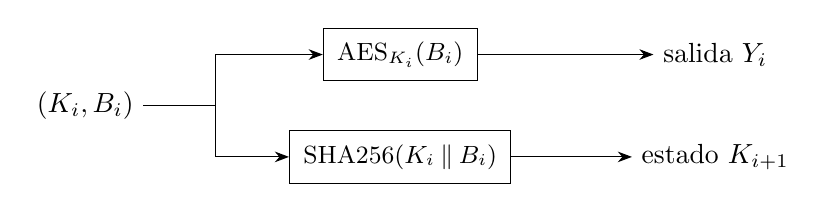
\begin{tikzpicture}[x=1cm,y=1cm]
\node (a) at (0,0) {\((K_i,B_i)\)};
\node[op] (enc) at (4,.65) {\(\Enc_{K_i}(B_i)\)};
\node[op] (hash) at (4,-.65) {\(\HH(K_i\cat B_i)\)};
\node (y) at (8,.65) {salida \(Y_i\)};
\node (k) at (8,-.65) {estado \(K_{i+1}\)};
\draw (a.east)--(1.65,0); \draw[arr] (1.65,0)|-(enc.west); \draw[arr] (1.65,0)|-(hash.west);
\draw[arr] (enc)--(y); \draw[arr] (hash)--(k);
\end{tikzpicture}
\caption{Funciones de salida y transición de estado en AES/SHA. La clave almacenada se sustituye después de calcular ambas ramas.}\label{fig:ais}
\end{figure}

El §996 permite cualquier valor fijo de \(p\). Se adopta \(p=0^{128}\), con lo que \(B_i=A_i\). Si sólo el último bit de \(p\) fuese uno, un bloque físico terminado en \texttt{ff} pasaría a terminar en \texttt{fe}. Esto cambia ambos resultados de~\eqref{eq:ais}, pero la transformación \(A_i\mapsto B_i\) sigue siendo invertible. El parámetro \(p\) puede ser público y no consume bits del extractor en cada petición.

\par\noindent\begin{minipage}{\linewidth}\small
\begin{verbatim}
Inicializar_AES_SHA():
    T0 = tomar128(Toeplitz)
    T1 = tomar128(Toeplitz)
    K  = concatenar(T0, T1)

Generar_AES_SHA():
    A = tomar128(Toeplitz)
    B = xor(p, A)
    Y = AES256_cifrar(clave=K, bloque=B)
    K = SHA256(concatenar(K, B))
    devolver Y
\end{verbatim}
\end{minipage}\par

\subsection{Tupla de AIS y longitud de petición}
La ecuación (3.1) del §129 describe un DRNG mediante la tupla
\((S,S_{\rm req},R,A,I,\phi,\phi_{\rm req},\phi_0,\psi)\).
La tabla~\ref{tab:tupla} especializa las definiciones del §997. \(S\) representa el estado que subsiste entre peticiones y \(S_{\rm req}\) el estado temporal de una petición. Este último contiene los operandos actuales como par lógico. Su anchura no aumenta la longitud de la clave ni implica que se necesite un segundo registro físico para almacenarla.
\begin{table}[htbp]\centering\small
\caption{Componentes de la tupla AES/SHA definida en AIS §§129 y 996--997.}\label{tab:tupla}
\begin{tabularx}{\linewidth}{@{}l l X@{}}\toprule
Símbolo & Función en el modelo & Especificación\\\midrule
\(S\)& Estado persistente & \(\bits^{256}\), con \(s=K_i\).\\
\(S_{\rm req}\)& Estado temporal & \(\bits^{256}\times\bits^{128}\), con \(u=(s,\iota(a))\).\\
\(R\)& Números internos & \(\bits^{128}\), el conjunto de bloques AES.\\
\(A\)& Entrada adicional & Cadenas de longitud de 0 a 128 bits en AIS; 128 bits en la interfaz física.\\
\(I\)& Longitudes de petición & El §996 establece el máximo de 128 bits. El perfil implementa \(I=\{128\}\).\\
\(\phi\)& Estado siguiente & \(\HH(s\cat(p\oplus\iota(a)))\).\\
\(\phi_{\rm req}\)& Preparación & \(\phi_{\rm req}(s,a)=(s,\iota(a))\).\\
\(\phi_0\)& Transición interna & \(\phi_0(u)=u\), pues se genera una sola palabra por petición.\\
\(\psi\)& Salida & \(\psi(s,\iota(a))=\Enc_s(p\oplus\iota(a))\).\\\bottomrule
\end{tabularx}
\end{table}

La longitud de petición \(L\) es el número de bits solicitados; la longitud de entrada \(\ell\) es el número de bits de \(a\). La palabra interna tiene una longitud fija \(k=128\). El §131 prevé \(\lceil L/k\rceil\) palabras internas. El §976 limita \(L\le k\) en esta familia de ejemplos, de modo que basta una evaluación de \(\psi\). Esta simplificación es compatible con el máximo general de \(2^{19}\) bits de DRG.3.2. Si se solicitasen sólo 64 bits, el prefijo de salida tendría \(2^{64}\) preimágenes físicas para una clave fija. Para entregar 256 bits se ejecutan dos peticiones completas, con actualización intermedia de la clave. Repetir \(\psi\) sobre el mismo estado temporal duplicaría la primera palabra.

El relleno \(\iota\) también determina el dominio de la prueba: las cadenas de bits \(1\) y \(10\) producen el mismo bloque rellenado. La biyección se demuestra para entradas de \emph{exactamente} 128 bits. El §996 representa la entrada ausente mediante ceros, por lo que una llamada sin entrada nueva produciría \(\Enc_{K_i}(p)\). El puerto físico admite 128 ceros cuando proceden efectivamente del extractor y espera cuando éste carece de una nueva palabra.

\subsection{Resiembra y tasa de salida}
AIS §384 permite incorporar los números intermedios por resiembra, como entrada adicional o mediante ambos mecanismos. El §390(iii) de la referencia técnica del BSI estudia expresamente la entrada adicional de 128 bits en esta construcción y concluye que se cumple PTG.3.4 con razón de compresión uno. Tras la siembra inicial, el perfil de la ecuación~\eqref{eq:ais} consume un bloque por salida y actualiza la clave en cada petición.

La variante experimental con resiembra periódica reserva dos bloques adicionales \(R_0,R_1\) y calcula \(K\gets K\oplus(R_0\cat R_1)\) antes de la siguiente generación. La resiembra incorpora el estado vigente y requiere que el material fresco satisfaga por sí mismo el crédito de entropía exigido (§148). Con una resiembra cada \(n\) entregas, la fracción útil del caudal intermedio es \(n/(n+2)\), suponiendo capacidad de cómputo suficiente. La elección comparativa \(n=1024\) coincide con \(2^{17}\) bits por época y con el límite de determinadas construcciones NIST basadas en CTR. AIS no establece esa periodicidad para el perfil de §390(iii).

\section{CTR\_DRBG con entrada física}\label{sec:ctr}
\subsection{Estado de trabajo, actualización e instanciación}
CTR\_DRBG es el mecanismo de generación determinista en modo contador definido en NIST SP 800-90A Rev.~1 \cite[§10.2.1]{nist90a}. AES cifra valores sucesivos de un contador y un procedimiento denominado \texttt{Update} modifica el estado. Se adopta AES-256 a fuerza de seguridad de 256 bits, sin función de derivación (\emph{no DF}), con campo de contador completo de 128 bits y sin resistencia a predicción bajo demanda. La personalización se fija a la cadena vacía. Esta modalidad de instanciación no requiere nonce.

El estado de trabajo se representa por \((K,V,r)\). \(K\) es la clave de 32 bytes y \(V\) el contador criptográfico de 16 bytes. \(r\) corresponde a \texttt{reseed\_counter} y permite comprobar el intervalo de resiembra; se incrementa una vez por petición. Los valores que se cifran con AES se obtienen incrementando \(V\), con aritmética módulo \(2^{128}\). También se conservan en el contexto los parámetros administrativos de la instancia.

Dado un argumento \(D\) de 384 bits, el procedimiento \(\upd(K,V;D)\) calcula tres bloques con la misma clave:
\begin{equation}
 G_j=\Enc_K((V+j)\bmod 2^{128}),\quad j=1,2,3,\qquad
 M=(G_1\cat G_2\cat G_3)\oplus D.
 \label{eq:update}
\end{equation}
Los primeros 256 bits de \(M\) forman la nueva clave y los últimos 128 bits forman el nuevo contador. Los tres cifrados son necesarios porque el par \((K,V)\) ocupa \(256+128=384\) bits y cada invocación de AES devuelve 128.

La instanciación consume 384 bits de material de siembra \(W\) con \emph{full entropy} en este perfil. Con personalización vacía se obtiene
\begin{equation}
 (K_0,V_0)=\upd(0^{256},0^{128};W),\qquad r_0=1 .
\end{equation}
Los registros de ceros son los operandos provisionales de la inicialización. El estado utilizado por la primera generación contiene el resultado de \texttt{Update}. Así se distingue el material recibido, \(W\), del estado derivado, \((K_0,V_0,1)\).

En la ruta NIST considerada, Toeplitz es el único acondicionador interno de la fuente y es \emph{non-vetted}. El procedimiento externo de \cite[§3.2.2.2]{nist90c} permite obtener \(W\) con AES-CMAC \cite{cmac}. La realización estudiada reserva seis bloques intermedios y calcula tres tags de 128 bits, uno por pareja, con la clave fija del acondicionador. Cada evaluación exige al menos \(128+64=192\) bits de entropía acreditada en su entrada. Los tres tags se concatenan. Si la fuente evaluada ya suministra entropía completa, los 48 bytes se pueden adquirir directamente. En ambos casos el primer bloque destinado a generación se consume después de la siembra, mediante una adquisición distinta.

\subsection{Generación y resiembra}
El argumento presente de entrada adicional es
\begin{equation}
 D_i=0^{256}\cat A_i,\qquad |A_i|=128 .
 \label{eq:input}
\end{equation}
Se entregan los 48 bytes completos a la interfaz de \texttt{Generate}. El primer \texttt{Update} incorpora \(D_i\), después se cifra un único contador y, por último, se vuelve a ejecutar \texttt{Update} con \(D_i\) a partir del contador ya incrementado. La figura~\ref{fig:ctr} distingue los estados intermedios. El resultado \(Y_i\) se devuelve con la transición completada.

\begin{figure}[htbp]\centering
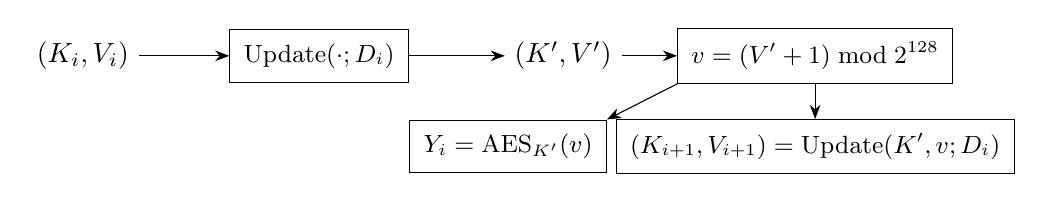
\begin{tikzpicture}[x=1cm,y=1cm]
\node (s) at (0,0) {\((K_i,V_i)\)};
\node[op] (u) at (3,0) {\(\upd(\cdot;D_i)\)};
\node (p) at (6.1,0) {\((K',V')\)};
\node[op] (inc) at (9.3,0) {\(v=(V'+1)\bmod 2^{128}\)};
\node[op] (e) at (5.4,-1.15) {\(Y_i=\Enc_{K'}(v)\)};
\node[op] (post) at (9.3,-1.15) {\((K_{i+1},V_{i+1})=\upd(K',v;D_i)\)};
\draw[arr] (s)--(u); \draw[arr] (u)--(p); \draw[arr] (p)--(inc);
\draw[arr] (inc.south west)--(e.north east); \draw[arr] (inc)--(post);
\end{tikzpicture}
\caption{Orden de operaciones para una petición CTR\_DRBG de 128 bits. La generación y la actualización posterior usan el mismo valor \(v\).}\label{fig:ctr}
\end{figure}

\par\noindent\begin{minipage}{\linewidth}\small
\begin{verbatim}
Generar_CTR():
    si r > intervalo_de_resiembra: devolver RESEED_REQUIRED
    A = tomar128(Toeplitz)
    D = concatenar(32 bytes cero, A)
    (Ktmp, Vtmp) = Update(K, V; D)
    v = (Vtmp + 1) mod 2^128
    Y = AES256_cifrar(clave=Ktmp, bloque=v)
    (K, V) = Update(Ktmp, v; D)
    r = r + 1
    devolver Y
\end{verbatim}
\end{minipage}\par

El coste de generación es de siete cifrados AES por palabra física: tres para la primera actualización, uno para la salida y tres para la actualización posterior. Se consume una sola palabra física de datos. En una resiembra se adquieren otros 48 bytes de entropía completa \(W\), se fija a vacía la entrada adicional de \texttt{Reseed}, se calcula \((K,V)\gets\upd(K,V;W)\) y se restablece \(r=1\). Para el perfil sujeto a SP 800-90C §5.3(6) se requiere resiembra antes de generar de nuevo una vez alcanzados \(2^{17}\) bits. Con 128 bits por petición se obtienen 1.024 peticiones entre siembras. Esta restricción corresponde a la construcción NIST aplicable.

\subsection{Posición de la entrada adicional}
Al aplicar~\eqref{eq:update} con~\eqref{eq:input}, los primeros 256 bits de \(D_i\) dejan intactos \(G_1,G_2\), y los últimos 128 se combinan con \(G_3\). En consecuencia,
\begin{equation}
 K'=G_1\cat G_2,\qquad V'=G_3\oplus A_i,\qquad
 Y_i=\Enc_{K'}((V'+1)\bmod 2^{128}).
 \label{eq:ctr}
\end{equation}
Fijado el estado previo, \(K'\) y \(G_3\) quedan determinados antes de incorporar \(A_i\). Esta ubicación del bloque permite la inversión de la sección~\ref{sec:its}.

Una entrada de sólo 16 bytes produciría otro resultado: SP 800-90A rellena por la derecha, de modo que los bits físicos entrarían en el campo de la clave. Con DF, el argumento se procesaría antes de \texttt{Update} y sería necesario analizar un mapa diferente. Si \(A_i=0^{128}\), se suministra un argumento \emph{presente} de 384 ceros; la cadena ausente omite la actualización previa. Para estado fijo, una petición de 256 bits con un solo \(A_i\) puede alcanzar a lo sumo \(2^{128}\) cadenas, lo que da distancia al menos \(1-2^{-128}\) a la uniforme de 256 bits. El perfil usa una nueva palabra física y una transición completa por cada 128 bits entregados.

\subsection{Tupla de generación y caudal}
En la notación del §129 de AIS, la tupla del núcleo CTR es
\((S,S_{\rm req},R,A,I,\phi,\phi_{\rm req},\phi_0,\psi)\), con
\[
 S=S_{\rm req}=\bits^{256}\times\bits^{128},\quad R=\bits^{128},\quad
 A=\{\emptyset\}\cup\bits^{128},\quad I=\{128\}.
\]
Aquí \(s=(K,V)\) denota el estado criptográfico y \(\operatorname{inc}(v)=(v+1)\bmod 2^{128}\). Se escribe \(\upd(s;D)\) como abreviatura de \(\upd(K,V;D)\). El contador administrativo \(r\) controla la admisión de la petición antes de ejecutar el núcleo. La entrada ausente se incluye para describir la ejecución autónoma que examina AIS. La interfaz de salida física utiliza siempre la rama de entrada presente. Las cuatro funciones son
\begin{align*}
 \phi_{\rm req}(s,a)&=
 \begin{cases}s & a=\emptyset,\\
 \upd(s;0^{256}\cat a)& |a|=128,\end{cases}
 &\phi_0(u)&=u,\\
 \psi(k,v)&=\Enc_k(\operatorname{inc}(v)),&
 \phi(s,a)&=\upd((k,\operatorname{inc}(v));D(a)),
\end{align*}
donde \((k,v)=\phi_{\rm req}(s,a)\), \(D(\emptyset)=0^{384}\) y \(D(a)=0^{256}\cat a\) para una entrada presente. La preparación determina la clave y el contador usados por la función de salida. La transición persistente usa el contador ya incrementado. Esta tupla se deriva de las operaciones de SP 800-90A para el perfil elegido.

Sea \(R_T\) el caudal disponible a la salida de Toeplitz, en bits por segundo. En régimen estacionario, si el cómputo alcanza esa velocidad y los únicos consumos adicionales son las resiembras periódicas, AES/SHA sin resiembra periódica entrega \(R_T\). Para CTR con \(n=1024\) peticiones por época, la ruta CMAC reserva seis bloques de Toeplitz por resiembra y entrega \(R_T n/(n+6)\). Con siembra directa de entropía completa la expresión pasa a \(R_T n/(n+3)\). Por ejemplo, para \(R_T=1\) Gbit/s se obtienen respectivamente 1.000, 994,17 y 997,08 Mbit/s. Si el gigabit por segundo se mide antes de Toeplitz y el extractor produce \(m\) bits por cada \(d\) bits crudos, estas cifras se multiplican por \(m/d\), suponiendo el mismo régimen y un suministro independiente de los selectores. El balance cuenta bits de interfaz. La garantía de entropía de los bloques entregados se calcula a continuación a partir de su distribución conjunta.

\section{Conservación de la aleatoriedad}\label{sec:its}
Sea \(X=(A_0,\ldots,A_{q-1})\) la secuencia de bloques físicos para un número fijo \(q\) de peticiones, e \(Y=(Y_0,\ldots,Y_{q-1})\) la secuencia emitida. Sea \(Z\) una variable clásica que recoge la información lateral considerada y determina el estado inicial. La política y el material de eventuales resiembras pueden incluirse en \(Z\) cuando se atraviesan sus fronteras. Se comparan las leyes de entrada y salida respecto del mismo \(Z\).

\begin{proposicion}\label{prop:causal}
Para los perfiles de las secciones~\ref{sec:ais} y~\ref{sec:ctr}, y para cada valor fijado \(z\), la transformación \(F_z:X\mapsto Y\) es una permutación de \(\bits^{128q}\).
\end{proposicion}
\begin{proof}
En AES/SHA, de~\eqref{eq:ais} se recupera un único valor de entrada a partir del estado previo \(K_i\) y de \(Y_i\):
\begin{equation}
 A_i=p\oplus\Enc^{-1}_{K_i}(Y_i).
 \label{eq:invais}
\end{equation}
El descifrado es la inversa definida para cada clave en FIPS 197 \cite{aes}. Sustituyendo el valor obtenido en \(K_{i+1}=\HH(K_i\cat(p\oplus A_i))\) se reconstruye el estado siguiente mediante una evaluación directa de SHA-256.

En CTR\_DRBG, el estado previo permite calcular \(G_1,G_2,G_3\) y \(K'\). La inversión de~\eqref{eq:ctr} da
\begin{equation}
 A_i=G_3\oplus\bigl((\Enc^{-1}_{K'}(Y_i)-1)\bmod 2^{128}\bigr).
 \label{eq:invctr}
\end{equation}
Después del descifrado se deshace el incremento y, finalmente, el XOR con \(G_3\). El valor recuperado determina \(D_i\) y permite ejecutar la actualización posterior con los mismos operandos que en la generación original.

Para invertir una secuencia completa se inicia el cálculo con el estado determinado por \(z\). En cada índice se recupera la única entrada mediante~\eqref{eq:invais} o~\eqref{eq:invctr}, se reconstruye el estado posterior y se incorpora la resiembra prevista, si procede. Por inducción, al principio de la petición \(i+1\) se dispone del estado que producirían las \(i+1\) entradas ya reconstruidas. El procedimiento se aplica a cualquier secuencia de salida, por lo que establece simultáneamente la inyectividad y la sobreyectividad.
\end{proof}

\begin{proposicion}\label{prop:medidas}
Sea \(U\) la ley uniforme en \(\bits^{128q}\). Los dos perfiles conservan la distancia de variación total a la uniforme y la minentropía condicional:
\[
 \Delta(P_{Y,Z},U\otimes P_Z)=\Delta(P_{X,Z},U\otimes P_Z),
 \qquad H_{\min}(Y\mid Z)=H_{\min}(X\mid Z).
\]
\end{proposicion}
\begin{proof}
Con \(N=2^{128q}\), la proposición~\ref{prop:causal} implica
\(P_{Y,Z}(y,z)=P_{X,Z}(F_z^{-1}(y),z)\). El cambio de índice \(y=F_z(x)\) en cada suma da
\[
 \tfrac12\sum_{z,y}|P_{Y,Z}(y,z)-P_Z(z)/N|
 =\tfrac12\sum_{z,x}|P_{X,Z}(x,z)-P_Z(z)/N|.
\]
La misma permutación preserva el máximo de cada fila \(z\). Así,
\(\sum_z\max_y P_{Y,Z}(y,z)=\sum_z\max_x P_{X,Z}(x,z)\).
Esta cantidad es la probabilidad óptima de adivinación. Su logaritmo negativo en base dos es la minentropía condicional.
\end{proof}

Para ilustrar el cambio de índice, considérese una permutación de dos bits que envía \((00,01,10,11)\) a \((01,11,00,10)\), respectivamente. Si las probabilidades de entrada, en orden binario, son \((1/2,1/4,1/8,1/8)\), las de salida en ese mismo orden son \((1/8,1/2,1/8,1/4)\). El valor más probable cambia de \(00\) a \(01\) y su probabilidad sigue siendo \(1/2\). En ambos casos la minentropía es un bit y la distancia a la uniforme es \(1/4\). En las dos construcciones estudiadas se aplica este mismo cambio de índice a la secuencia completa, una vez fijado el contexto.

\paragraph{Siembra procedente del mismo extractor.}
Sea \(C\) el prefijo de Toeplitz reservado a la siembra y \(E\) la información lateral frente a la cual se ha caracterizado el flujo físico. En AES/SHA, \(C\) comprende los dos primeros bloques. En CTR con CMAC para siembra comprende los seis bloques utilizados para obtener \(W\). En ambos casos, \(C\) determina el estado inicial. Aunque la preparación de \(W\) comprima el prefijo, el mapa \((c,x)\mapsto(c,F_c(x))\) es una permutación sobre el flujo completo: deja fijo el prefijo e invierte la parte destinada a datos. Si \((C,X,E)\) está a distancia a lo sumo \(\varepsilon\) de \(U_C\otimes U\otimes P_E\), se sigue que
\[
 \Delta(P_{C,Y,E},U_C\otimes U\otimes P_E)
 =\Delta(P_{C,X,E},U_C\otimes U\otimes P_E)\le\varepsilon.
\]
Descartar \(C\) en ambas distribuciones da \(\Delta(P_{Y,E},U\otimes P_E)\le\varepsilon\). El posprocesamiento no añade error por llamada. Si la premisa disponible consiste en cotas \(\delta_i\) de distancia de cada bloque a la uniforme condicionada a todo historial admisible y a la información lateral, la regla de la cadena y la desigualdad triangular permiten tomar \(\varepsilon\le\sum_i\delta_i\) para los bloques así caracterizados.

\paragraph{Información lateral cuántica y verificación formal.}
Para un registro lateral cuántico, la permutación del registro clásico, controlada por el contexto clásico que determina el estado inicial, deja invariante el estado ideal y preserva la distancia de traza por invariancia unitaria. Al reindexar los resultados de cada medición se preserva también la probabilidad óptima de adivinación. Las declaraciones \leanlink{37}{aisRun} y \leanlink{43}{ctrRun} en Lean enlazan las funciones de generación con su ejecución secuencial. \leanlink{53}{aisITS} y \leanlink{61}{ctrITS} formalizan las identidades clásicas; \leanlink{79}{aisCQ} y \leanlink{87}{ctrCQ} verifican la reindexación bajo las leyes de operadores del modelo clásico-cuántico. El alcance de estas pruebas comprende los perfiles algorítmicos indicados y las hipótesis explícitas sobre sus primitivas.

\paragraph{Hipótesis sobre las primitivas.}
La biyectividad es necesaria y suficiente para que una función determinista, entre alfabetos del mismo tamaño, conserve la uniformidad de toda entrada uniforme. Para un alfabeto de tamaño \(N\), la masa de salida en \(y\) es \(|f^{-1}(y)|/N\). Una permutación conserva, además, las masas de cualquier otra distribución. Aplicado por estado, este resultado sólo exige que la transición siguiente se pueda calcular a partir del estado anterior y de la entrada recuperada. En particular, una actualización constante en lugar de SHA conservaría la proposición~\ref{prop:medidas}. Sin embargo, eliminaría la influencia de la entrada física sobre el estado y haría constante la secuencia autónoma después de la primera transición. Por otra parte, si todas las entradas físicas se fijan a cero y se suprimen las resiembras, tres salidas consecutivas quedan determinadas por los 256 bits de \(K_0\). El soporte tiene a lo sumo \(2^{256}\) elementos entre \(2^{384}\) cadenas posibles. La seguridad computacional que pueda ofrecer la ejecución autónoma es compatible con esa limitación de entropía.

\section{Condiciones sobre la información lateral y comparación con Hash\_DRBG}
Los siguientes ejemplos precisan el alcance de la proposición~\ref{prop:medidas}. El primero considera una entrada marginalmente uniforme correlacionada con la clave inicial. Para \(p=0\), sean \(k_0=0^{256}\), \(k_1=0^{255}1\) y \(A\) uniforme en \(N=2^{128}\) valores. Se fija \(K=k_1\) si \(A=0^{128}\) y \(K=k_0\) en otro caso. Con AES-256 se obtiene
\begin{align*}
 \Enc_{k_0}(0^{128})=y_0&=\mathtt{dc95c078a2408989ad48a21492842087},\\
 \Enc_{k_1}(0^{128})=y_1&=\mathtt{6b6cfe160a6263631b292f879eeff926},\\
 \Enc^{-1}_{k_0}(y_1)&=\mathtt{4a68caef64fb37013c20d9a598089463}.
\end{align*}
Respecto de la permutación con clave \(k_0\), se modifica una sola entrada. \(y_0\) carece de preimagen y \(y_1\) tiene dos. Por tanto \(\Delta(P_Y,U)=1/N\) y \(H_{\min}(Y)=127\), aun siendo \(A\) marginalmente uniforme. La igualdad del teorema se mantiene al condicionar entrada y salida a \(K\).

Análogamente, un bloque de 128 bits elegido uniformemente entre las palabras de paridad par tiene bits marginalmente uniformes y minentropía de 127 bits, pero dista \(1/2\) de la distribución uniforme de 128 bits. Una secuencia de \(q\) copias de un mismo bloque uniforme dista \(1-2^{-128(q-1)}\) de la uniforme de \(128q\) bits. Estos ejemplos explican por qué la garantía admitida en la sección~1 se refiere a la distribución conjunta del flujo.

La exposición posterior del estado también cambia la información lateral. Para \(K=0^{256}\), \(p=0\) y un bloque uniforme \(A\), sea \(h(a)=\HH(K\cat a)\). Si se revela \(H=h(A)\), cada valor alcanzable de \(H\) contribuye \(1/N\) a la probabilidad de adivinación de \(A\) conociendo \(H\). En consecuencia \(p_{\rm guess}(A\mid H)=|\operatorname{Im}h|/N\). Los sufijos de 16 bytes correspondientes a los enteros cero y uno producen resúmenes distintos. De ello se deduce \(H_{\min}(A\mid H)\le127\). La igualdad frente a esa misma fuga subsiste para \(Y\), pero la garantía anterior a la exposición puede ser mayor. En CTR, conocer el estado anterior y la primera mitad de la clave posterior permite reconstruir el bloque emitido \cite{expediente}.

\subsection{Hash\_DRBG con SHA-256}
Para el mecanismo Hash\_DRBG de SP 800-90A, el registro \(V\) tiene 440 bits cuando se usa SHA-256. Si la entrada adicional \(A\) está presente y se solicitan \(r\le256\) bits, la generación del primer bloque se reduce a
\[
 W=\HH(\mathtt{02}\cat V\cat A),\quad V'=(V+W)\bmod 2^{440},
 \quad Y=\operatorname{prefijo}_r(\HH(V')) .
\]
El octeto \texttt{02} separa el dominio del primer hash. \(V'\) se serializa en 55 bytes para el segundo. La conservación exacta de una entrada uniforme de \(r\) bits exigiría una preimagen por cada salida para cada estado fijo. La resistencia computacional a colisiones de SHA-256 no determina ese número de preimágenes.

Un ejemplo reproducible fija \(V\) mediante \texttt{Hash\_df}: el material de entropía de prueba contiene los 32 octetos \texttt{00} a \texttt{1f}, el nonce contiene los octetos \texttt{20} a \texttt{2f} y la personalización es vacía. Se fija \(r=8\) y se enumeran los 256 valores de un octeto adicional desde el mismo estado. Se alcanzan 166 salidas; el octeto \texttt{86} tiene las seis preimágenes \texttt{0a}, \texttt{6f}, \texttt{9a}, \texttt{b3}, \texttt{d7} y \texttt{e7}. Como seis es la multiplicidad máxima, se obtiene \(H_{\min}(Y\mid V)=8-\log_2 6\simeq5.415\) y \(\Delta(P_{Y\mid V},U_8)=90/256\). La colisión corresponde al prefijo emitido. La enumeración refuta la conservación universal en la interfaz; para el perfil de 128 bits no establece la existencia de una colisión concreta. La evaluación DRG.3 de Hash\_DRBG en AIS §§1033--1075 atañe a otras propiedades.

\section{Interpretación normativa}\label{sec:norma}
\subsection{DRG.3 y PTG.3}
El §998 de AIS reconoce la conformidad DRG.3 del ejemplo AES/SHA del §996 y apoya su argumento en la seguridad criptográfica de AES-256 y en la unidireccionalidad de la transición SHA-256. El §397(ii) reconoce la conservación de entropía para un posprocesamiento biyectivo a estado fijo. La transcripción de los §§996--998 figura en el apéndice~\ref{app:bsi}. Las obligaciones correspondientes a una instancia concreta son las siguientes \cite[§§129--148, 207--214 y 380]{ais}.

\begin{description}
\item[DRG.3.1 y .4.] Se deben acreditar el origen de la siembra o resiembra y la entropía inicial efectiva. En la opción seleccionada el material procede de un PTG.2 y se exige minentropía efectiva de al menos 240 bits. La concatenación inicial conserva la distribución conjunta de los dos bloques; la reserva de bloques diferentes, por sí sola, no acredita su calidad conjunta.
\item[DRG.3.2 y .3.] El límite de petición se cumple por \(128\le2^{19}\). Para el estado efectivo se requieren al menos 246 bits. En AES/SHA, comparar las respuestas de cada clave a cinco textos fijos separa sus clases de comportamiento bajo la hipótesis de firmas distintas. La cardinalidad del registro, el soporte de siembra y la dificultad computacional de inferir la clase efectiva son magnitudes diferentes.
\item[DRG.3.5 y .6.] Se evalúa la predicción del sucesor o el predecesor de una ventana de salidas observadas. El §998 fundamenta la dificultad de predicción en AES con clave desconocida. El análisis debe incorporar la dependencia de las claves sucesivas a través de SHA-256.
\item[DRG.3.7 y .8.] La protección de salidas anteriores se evalúa concediendo el estado posterior y, según proceda, la última entrada. La elección adversaria de la entrada adicional, incluida la vacía, debe quedar cubierta. Según §211, la dificultad algorítmica exigida debe subsistir aun sin aportación de entropía física.
\item[DRG.3.9 y .10.] Se requieren funciones criptográficas de transición y salida, unidireccionalidad de la transición e inconspicuidad estadística. El análisis de preimágenes de \(\HH(s\cat b)\) distingue el sufijo conocido del caso en que se permite elegirlo. Las pruebas estadísticas aplicables y su justificación se rigen por §§200 y 209.
\end{description}
En el análisis cuantitativo de AES/SHA se fija un texto \(b\) determinado por el historial autorizado. Para una clave uniforme \(K\), la hipótesis de seguridad se formula sobre la pareja \((\Enc_K(b),\HH(K\cat b))\). Una ventaja de sustitución por uso acotada por \(\alpha(T)\), para observadores de coste \(T\) que incluyen la simulación restante, da por composición una cota \(2^{-t}+n\alpha(T)\) para el acierto sobre \(t\) bits ocultos en \(n\) peticiones, limitada a uno. La reducción requiere justificar la hipótesis sobre la pareja de primitivas, el horizonte de análisis y la distribución de la siembra. Las proposiciones~\ref{prop:causal} y~\ref{prop:medidas} son independientes de tales hipótesis \cite{expediente}.

Para CTR, el §1007 atribuye al solicitante la demostración para su configuración. Las ecuaciones de la sección~\ref{sec:ctr} establecen la correspondencia con la generación de NIST y la inversa frente al dato físico. El expediente obtiene una cota de clases de comportamiento en el modelo de cifrado ideal y desarrolla una reducción para predicción e inversión. Para AES concreto y el horizonte de 1.024 peticiones sigue abierta la justificación computacional cuantitativa de DRG.3.3 a 246 bits mediante esa reducción. La prueba ITS del perfil permanece válida.

\subsection{Integración del generador físico}
PTG.3.2 remite a DRG.3.3 y .5--.8 para el comportamiento algorítmico autónomo (§380). El §381 exige que el intermedio influya en el estado posterior. AES/SHA lo incorpora mediante SHA-256; CTR lo incorpora en ambas actualizaciones. La correspondencia entre estas transiciones y el equipo debe verificarse para el conjunto de estados admitidos. El §383 exige secreto, autenticidad e integridad de los intermedios. Esto afecta a la protección de las colas, el acceso de diagnóstico y el borrado del estado temporal (§§131 y 134). Ante dos peticiones simultáneas o un reinicio durante la actualización debe quedar determinado qué bloque se consumió, qué estado quedó vigente y si la salida llegó a emitirse.

La reutilización de una evaluación PTG.2 está sujeta a sus condiciones documentadas (§401). Para Toeplitz con selección aleatoria de la función, §338(a--f) establece condiciones sobre la elección e incidencia de selectores desfavorables, la ley fuerte aplicable a sus calidades, el secreto del índice, el tamaño de la familia y la dependencia entre índices. En el diseño típico con PTG.2 interno y transformación biyectiva 1:1, §398 limita las afirmaciones cuantitativas internas de PTG.3.5 a \(v_m=0.98\) para minentropía y \(v_S=0.9998\) para entropía de Shannon. El §399 reconoce la sexta opción para §390(iii) cuando se acreditan ambas condiciones. Una garantía ITS conjunta adicional se expresa frente a su propia información lateral y horizonte.

Las condiciones de puesta en marcha, ensayos en línea y respuesta a fallo total se aplican conforme a PTG.3.6--.8. Para el caso 1 de §417, el análisis debe contemplar qué intermedios dependen de muestras de datos o de selector adquiridas desde el fallo físico, incluida la latencia de detección. La generación cesa cuando se agotan los intermedios admisibles. El §422 sitúa la batería \(T_{\rm irn}\) en el PTG.2 de este diseño. Los §§423 y 200 cubren la justificación de PTG.3.9 para la salida final.

\subsection{Alcance de SP 800-90C}
El acceso directo a \texttt{Generate} del mecanismo CTR se evalúa con los requisitos de RBG2(P) en el supuesto de §6.3(8) de SP 800-90C. La acreditación de entropía completa de \(W\) se refiere a la siembra. La declaración NIST de salida de un RBG3 requiere ejecutar una de las construcciones definidas en §§6.4 y 6.5. En RBG3(XOR), la palabra física se combina por XOR con la salida del DRBG. En RBG3(RS), se aporta material fresco mediante resiembra antes de generar. Cada ruta tiene su propio balance de entropía y su propia transición de estado. La igualdad ITS probada aquí corresponde al perfil directo de la ecuación~\eqref{eq:input} \cite{nist90c,expediente}.

\section{Conclusiones}
En ambos perfiles, cada bloque físico de 128 bits determina una única salida de 128 bits y es recuperable para un estado anterior conocido. La reconstrucción del estado siguiente permite extender esta propiedad a cualquier secuencia finita de peticiones completas, sin suponer independencia entre los bloques de entrada. La cota ITS del flujo de Toeplitz se conserva al incluir la siembra en el análisis. En el caso AES/SHA existe además un precedente normativo explícito para el uso de esa interfaz en PTG.3. Para CTR\_DRBG, la conformidad algorítmica DRG.3 y la calificación de entropía completa de la salida según NIST requieren las justificaciones específicas indicadas en la sección~\ref{sec:norma}.

\appendix
\section{Vectores de ejecución y reproducibilidad}\label{app:vectores}
Los vectores de la tabla~\ref{tab:vectores} emplean datos públicos. Los índices 0 y 1 denotan dos peticiones consecutivas. En AES/SHA se fija \(p=0^{128}\) y se siembra con los octetos consecutivos \texttt{00} a \texttt{1f}. En CTR se instancian los registros a partir de los 48 octetos consecutivos \texttt{00} a \texttt{2f}. Las entradas físicas comunes son
\begin{align*}
 A_0&=\mathtt{00112233445566778899aabbccddeeff},\\
 A_1&=\mathtt{ffeeddccbbaa99887766554433221100}.
\end{align*}
\begin{table}[htbp]\centering\small
\caption{Valores hexadecimales de estados y salidas. Dos líneas en una celda representan una sola cadena, por orden de lectura.}\label{tab:vectores}
\begin{tabular}{@{}lll@{}}\toprule
 & AES/SHA & CTR\_DRBG\\\midrule
\(K_0\) & \texttt{000102030405060708090a0b0c0d0e0f}&\texttt{530e88f8c34030bea16abefac8c67d84}\\
 &\texttt{101112131415161718191a1b1c1d1e1f}&\texttt{deb6522e59757d791f57dfc8a6ee8307}\\
\(V_0,\ r_0\)& --- & \texttt{524121e913830c53f98bdfa5592b1ba1}, 1\\
\(Y_0\)&\texttt{8ea2b7ca516745bfeafc49904b496089}&\texttt{3b92e82a937ba7edca937f53e6fba3f5}\\
\(K_1\)&\texttt{110a7585fc26c396520879d7319edb89}&\texttt{5add22fe81e86405ffb14cff50c43f78}\\
 &\texttt{a7fa5d70c558855d172f0c9bbe97d9ca}&\texttt{7a42489c241c9a169e385b6aa99350aa}\\
\(V_1,\ r_1\)& --- & \texttt{e55591e638a262f81eb2723dfab5d386}, 2\\
\(Y_1\)&\texttt{a393670043992fc25afe3dae37c29493}&\texttt{babd20902023a587c2478a42f0cd8e80}\\\bottomrule
\end{tabular}
\end{table}
El código de \texttt{experiments/profiles.py} implementa la instanciación y la generación de ambos perfiles. Los experimentos \texttt{its\_audit\_witness.py} y \texttt{hash\_drbg\_witness.py}, en el mismo directorio, reproducen los ejemplos de correlación, exposición del estado y multiplicidades de Hash\_DRBG. El archivo \texttt{formal/verification.json} registra las huellas de los módulos y el resultado de su verificación con Lean~4.19.0 \cite{expediente}.

\section{Texto original de AIS 20/31, versión 3.0, §§996--998}\label{app:bsi}
Transcripción de Peter y Schindler \cite[sección 5.2.2, pp.~203--204]{ais}. En la notación original, \(s\) es la clave \(K_i\) y el primer argumento de AES es el bloque \(p\oplus\iota(a)\). En el perfil físico, \(a=A_i\) ocupa 128 bits y \(\iota(a)=A_i\).
\begingroup
\small
\setlength{\parskip}{6pt}
\textbf{996}\quad [DRG.3-compliant DRNG with bijective output function] First, \(p\in\{0,1\}^{128}\) is a constant. The additional input \(a\in A\) is a bit string of length \(\ell\in\{0,\ldots,128\}\), and \(\iota(a):=(a,0\ldots,0)\in\{0,1\}^{128}\), i.e., \(\iota(\cdot)\) extends \(a\) to a 128-vector by appending 0's to the right. In particular, if \(a=\emptyset\) then \(\iota(a)=(0,\ldots,0)\). The output function \(\psi_{(b)}:\{0,1\}^{256}\times A\to\{0,1\}^{128}\) is given by \(\psi_{(b)}(s,a):=\text{AES-256}(p\oplus\iota(a),s)\). The key \(s\in\{0,1\}^{256}\) is the current internal state. The state transition function \(\phi_{(b)}:\{0,1\}^{256}\times A\to\{0,1\}^{256}\), \(\phi_{(b)}(s,a):=\text{SHA-256}(s\Vert p\oplus\iota(a))\). Following par.~976, we assume that requests are limited to 128 bits, which is the bit length of a single internal random number).

\textbf{997}\quad The describing 9-tuple reads as follows: \(S=\{0,1\}^{256}\), \(S_{\mathit{req}}=\{0,1\}^{256}\times\{0,1\}^{128}\), \(R=\{0,1\}^{128}\), \(A=\{a\in\{0,1\}^{*}\mid 0\le |a|\le 128\}\), \(\phi_{(b)}\) (state transition function), \(\phi_{\mathit{req}(b)}:S\times A\to S_{\mathit{req}}\), \(\phi_{\mathit{req}(b)}(s,a):=(s,\iota(a))\), \(\phi_0:S_{\mathit{req}}\to S_{\mathit{req}}\), \(\phi_0(s):=s\) (the definition of \(\phi_0\) is irrelevant because a request requires only one internal random number), and \(\psi_{(b)}:S_{\mathit{req}}\to R\) (output function).

\textbf{998}\quad [DRG.3-compliant DRNG with bijective output function, ctd.] We first note that the DRNG described in par.~996 is compliant with functionality class DRG.3: Both the state transition function \(\phi_{(b)}\) and the output function \(\psi_{(b)}\) are cryptographic. Finding predecessors or successors to a given sequence of internal random numbers \(r_i,\ldots,r_j\) would require that an adversary were able to mount a successful chosen-plaintext attack or chosen-ciphertext attack on AES-256, which is not considered practically feasible; cf. Subsection 5.2.1. The one-way function property of the state transition function \(\phi_{(b)}\) ensures enhanced backward secrecy.
\endgroup
\begin{thebibliography}{9}
\bibitem{ais} M. Peter y W. Schindler. \emph{A Proposal for Functionality Classes for Random Number Generators}. Versión 3.0, Bundesamt für Sicherheit in der Informationstechnik, 10 de septiembre de 2024. \href{https://www.bsi.bund.de/SharedDocs/Downloads/EN/BSI/Certification/Interpretations/AIS_31_Functionality_classes_for_random_number_generators_e_2024.pdf?__blob=publicationFile\&v=3\#page=211}{Texto oficial, §§996--998}.
\bibitem{aes} NIST. \emph{Advanced Encryption Standard (AES)}. FIPS 197-upd1, 2023. \url{https://doi.org/10.6028/NIST.FIPS.197-upd1}.
\bibitem{sha} NIST. \emph{Secure Hash Standard (SHS)}. FIPS 180-4, 2015. \url{https://doi.org/10.6028/NIST.FIPS.180-4}.
\bibitem{nist90a} E. Barker y J. Kelsey. \emph{Recommendation for Random Number Generation Using Deterministic Random Bit Generators}. NIST SP 800-90A Rev. 1, 2015. Tabla 3 y §§10.1.1, 10.2.1, 10.3.1. \url{https://doi.org/10.6028/NIST.SP.800-90Ar1}.
\bibitem{nist90c} NIST. \emph{Recommendation for Random Bit Generator (RBG) Constructions}. SP 800-90C, 2025. §§3.2.2.2, 5.3 y 6.3--6.5. \url{https://doi.org/10.6028/NIST.SP.800-90C}.
\bibitem{cmac} M. Dworkin. \emph{Recommendation for Block Cipher Modes of Operation: The CMAC Mode for Authentication}. NIST SP 800-38B, 2005, actualización de 2016. \url{https://doi.org/10.6028/NIST.SP.800-38B}.
\bibitem{expediente} \emph{Conservación de aleatoriedad física en dos diseños candidatos a PTG.3}. Expediente técnico, demostraciones en Lean y vectores experimentales. \href{https://github.com/jordiprga/technical-work/tree/2804a8b2bee6c6a5ac2a007d46a3eee56ecd7ecb/operation-token-burn-2026-11-14/00_coordination/ptg3-its}{Fuentes y resultados reproducibles}. Fuentes consultadas el 27 de noviembre de 2026.
\end{thebibliography}
\end{document}
